% moxi.tex:

\chapter{MOBILE-PHONE-BASED OXIMETER (MOXI)} % all caps please
\label{chap:moxi}
This is where the writing goes. 


\section{Introduction} %significan
\label{chap:moxi:introduction}
Every year, nearly 3 million newborns die within the first 4 weeks of life in \ac{LMIC}s~\cite{Worldhealthorganization2006}. Respiratory complications, such as birth asphyxia, and congenital heart defects, such as Tetralogy of Fallot (which results in Blue Baby Syndrome – a condition caused by low tissue oxygenation), are among the major causes of death at birth for neonates. In addition, over 17\% of the post-neonatal child deaths are caused by childhood pneumonia and other acute respiratory infections, accounting for 4 million deaths per year for children under age 5~\cite{Alexander2018}. These conditions often lead to low arterial and tissue oxygenation~\cite{Weber2003}. Many of these complications are easily screened, diagnosed, and continuously monitored in most facilities in developed countries using a pulse oximeter, a device to measure arterial blood oxygen levels (SpO2) using low-power light based on NIRS. 

Finger-clip-based pulse oximeters, however, are difficult to use on small fingers. Newborn specific pulse oximeter probes, often sold as disposable parts, can cost up to \$100 USD, and require a more expensive oximeter system to read and display results~\cite{Ouro-BangnaMaman2005,Heywood1989}. These designs thus have extremely limited presence in first-level clinics in LMICs. In recent years, portable NIR devices have been reported, but they generally have high costs dues to sensitive charge-coupled device (CCD) cameras and stand-alone image acquisition software~\cite{Jung2013}, or still require the use of a finger-clip~\cite{Karlen2011,Hudson2012}. Many factors, primarily high acquisition and maintenance costs (Table~\ref{tab:lmicbarriers}), have hindered the adoption of portable diagnostics tools~\cite{Malkin2007}. 

A silver lining comes from the Pew Global Research Center, which reported that smartphone ownership in \ac{LMIC}s rose from 21\% to 45\% between 2013 and 2018, making smartphone networks the fastest growing infrastructure in LMICs~\cite{Poushter2016}. By capitalizing on the ubiquitous presence of smartphones worldwide, we aim to develop phone-camera based and phone-communication facilitated NIRS devices to measure tissue oxygenation, directly addressing the barriers to adoption in Table~\ref{tab:lmicbarriers}. These smartphone-based devices can address the current limitations of conventional pulse oximeters, including newborn-unfriendly clip designs, acquisition and maintenance costs of disposable probes, and the need for frequent disinfection due to direct skin contact. Leveraging smartphone features such as cameras, LEDs, and wireless communication along with their power and computation will pave the way for POC smartphone-based diagnostic tools. 

\begin{table}[]
\centering
\caption{Barriers to adoption of new medical devices in LMICs}
\label{tab:lmicbarriers}
\begin{tabular}{@{}cl@{}}
\toprule
Rank & Barrier to Adoption \\ \midrule
1    & Acquisition Costs   \\
2    & Spare Parts         \\
3    & Consumables         \\
4    & Reliable Power      \\
5    & Infrastructure      \\
6    & Training            \\ \bottomrule
\end{tabular}
\end{table}

In this chapter, we establish the feasibility and accuracy of three smartphone-based approaches to monitoring oxygenation. In order of decreasing complexity of hardware, the first design (D1) is a Bluetooth wireless oximeter board with a dedicated pulse oximetry chip. The second design (D2) measures tissue oxygen saturation (StO2). It functions by imaging light attenuation in tissue through a slit on a circuit board carrying LEDs. The third design (D3) is a paper filter covering half of the field of view of a smartphone camera. Both D1 and D3 designs utilize our in-house developed mobile phone application to monitor heart rate (HR) and arterial oxygen saturation (SpO2). The three devices, along with a screenshot of the mobile phone application, are seen in the figure below. Although we include details on D1 and D2 for completeness, when we refer to the \ac{MOXI} system, we are referring to the D3 design. 

\begin{figure}
	\begin{center}
	\subfigure[]{\label{fig:moximeter}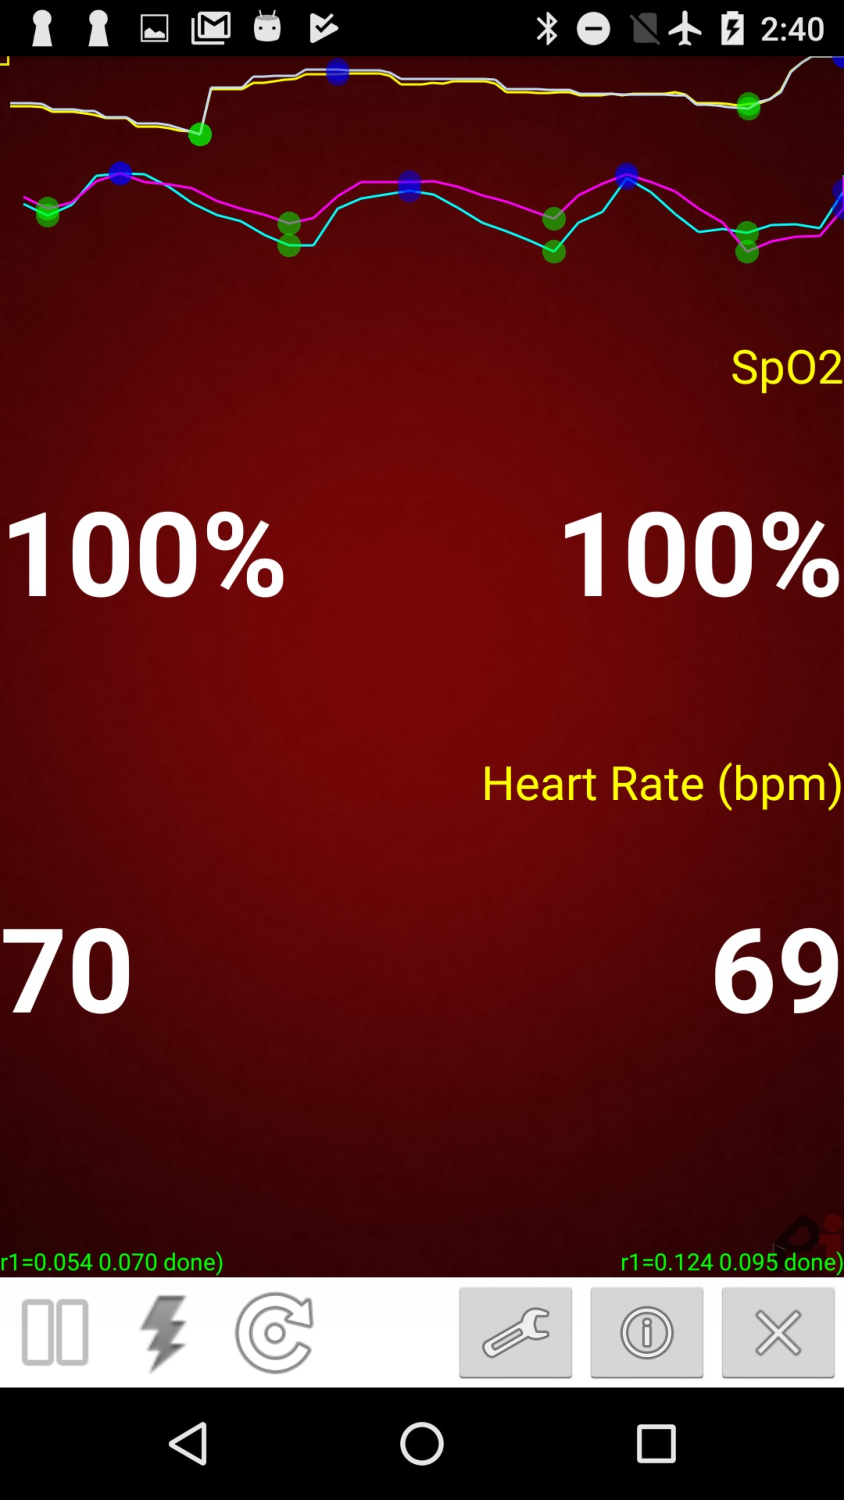
\includegraphics[height=5cm]{fig/moxi/moximeter.pdf}}
	\subfigure[]{\label{fig:D1D3}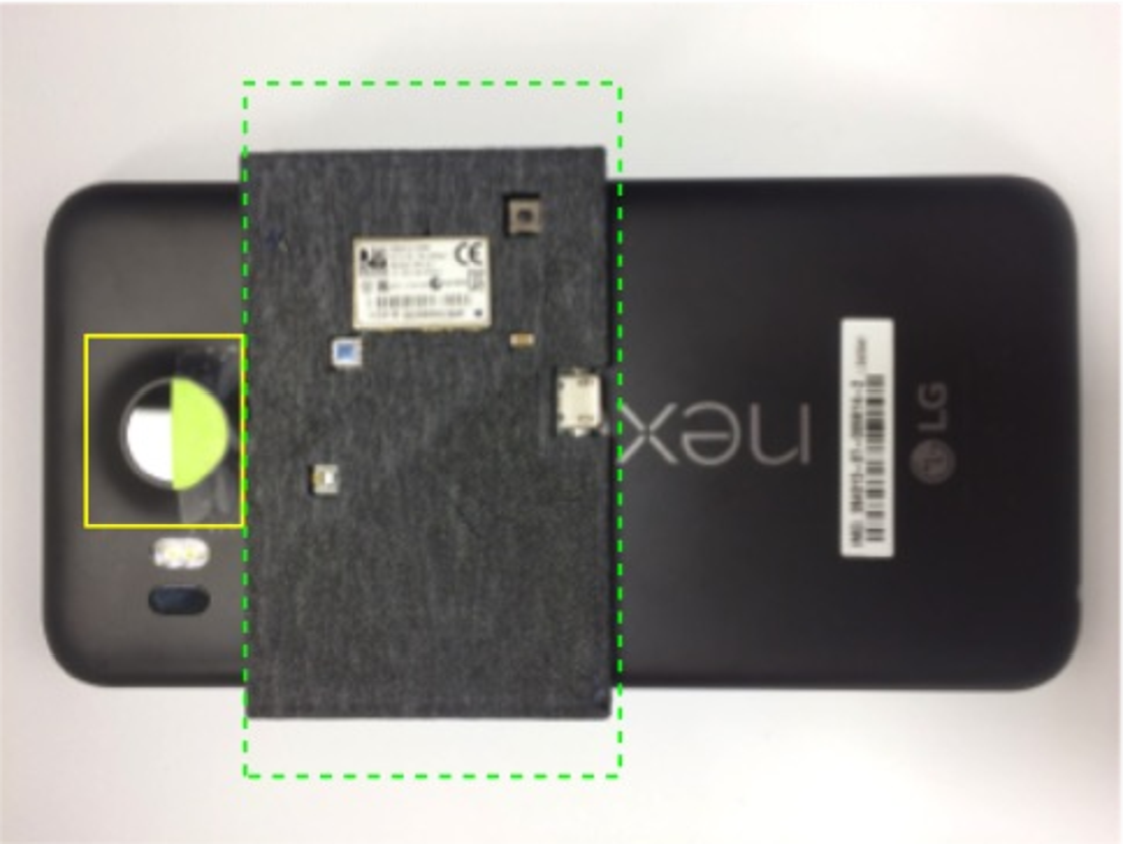
\includegraphics[height=5cm]{fig/moxi/D1D3.pdf}}
	\subfigure[]{\label{fig:D2}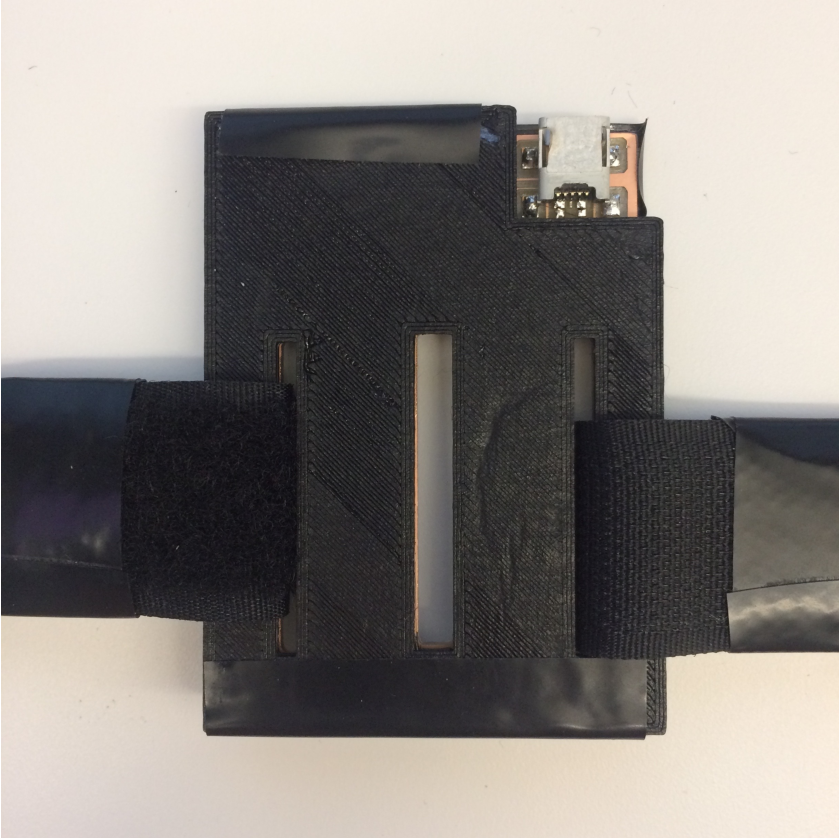
\includegraphics[width=5cm]{fig/moxi/D2.pdf}}
	\end{center}
	\caption{(a) Screenshot of Moximeter mobile application simultaneously capturing D1 and D3 data. (b) D1 (green, dashed) and D3 (yellow, solid) mounted on a smartphone phone. (c) D2 board with cover.} 
	\label{fig:designs}
\end{figure} 


\section{Methods}
\label{chap:moxi:methods}



\section{Results}
\label{chap:moxi:results}



\section{Discussion}
\label{chap:moxi:discussion}




% --- EOF ---